

\section{Overview}
  \begin{itemize}
    \item The Sequence Labeling (or Tagging) Problem
    \item Generative models, and the noisy-channel model, for supervised learning
    \item Hidden Markov Model (HMM) taggers
    \begin{itemize}\scriptsize
    \item Basic definitions
    \item Parameter estimation
    \item The Viterbi algorithm
    \end{itemize}
  \end{itemize}
 This slides are based on the course material by Michael Collins: \url{http://www.cs.columbia.edu/~mcollins/cs4705-spring2019/slides/tagging.pdf}


\section{Sequence Labeling or Tagging Tasks}

  \begin{itemize}
    \item Sequence Labeling or Tagging is a task in NLP different from document classification.
    \item Here the goal is to map a sentence represented as a sequence of tokens $x_1,x_2,\dots,x_n$ into a sequence of tags or labels $y_1,y_2,\dots,y_n$.
    \item Well known examples of this task are Part-of-Speech (POS) tagging and Named Entity Recognition (NER) to be presented next.
    \end{itemize}


\section{Part-of-Speech Tagging}
  \textcolor{green}{\textbf{INPUT:}}
  Profits soared at Boeing Co., easily topping forecasts on Wall Street, as their CEO Alan Mulally announced first quarter results.  \vspace{0.5cm}
  
  \textcolor{green}{\textbf{OUTPUT:}}
  Profits\textcolor{red}{/N} soared\textcolor{red}{/V} at\textcolor{red}{/P} Boeing\textcolor{red}{/N} Co.\textcolor{red}{/N} ,\textcolor{red}{/,} easily\textcolor{red}{/ADV} topping\textcolor{red}{/V} forecasts\textcolor{red}{/N} on\textcolor{red}{/P} Wall\textcolor{red}{/N} Street\textcolor{red}{/N} ,\textcolor{red}{/,} as\textcolor{red}{/P} their\textcolor{red}{/POSS} CEO\textcolor{red}{/N} Alan\textcolor{red}{/N} Mulally\textcolor{red}{/N} announced\textcolor{red}{/V} first\textcolor{red}{/ADJ} quarter\textcolor{red}{/N} results\textcolor{red}{/N} .\textcolor{red}{/.}
   \vspace{0.5cm}
  \begin{itemize}
    \item \textcolor{red}{N} = \textcolor{blue}{Noun}
    \item \textcolor{red}{V} = \textcolor{blue}{Verb}
    \item \textcolor{red}{P} = \textcolor{blue}{Preposition}
    \item \textcolor{red}{Adv} = \textcolor{blue}{Adverb}
    \item \textcolor{red}{Adj} = \textcolor{blue}{Adjective}
    \item ...
  \end{itemize}


  \begin{figure}[h]
        	\includegraphics[scale = 0.34]{pics/posTags.png}
        \end{figure}
Source: \cite{JurafskyBook}


\section{Named Entity Recognition (NER)}
A \textbf{named entity} is, roughly speaking, anything that can be referred to with a named entity proper name: a person, a location, an organization.\vspace{0.5cm}

  \textcolor{green}{\textbf{INPUT:}}
  Profits soared at Boeing Co., easily topping forecasts on Wall Street, as their CEO Alan Mulally announced first quarter results.    \vspace{0.5cm}

  \textcolor{green}{\textbf{OUTPUT:}}
  Profits soared at \textcolor{red}{[Company} Boeing Co.\textcolor{red}{]}, easily topping forecasts on \textcolor{red}{[Location} Wall Street\textcolor{red}{]}, as their CEO \textcolor{red}{[Person} Alan Mulally\textcolor{red}{]} announced first quarter results. \vspace{0.5cm}

  \begin{itemize}
   \item  Since entities can span multiple words (i.e., a span recognition problem), we can use BIO tagging \cite{ramshaw1999text} to turn the problem into a sequence labeling problem.
   \item   BIO tagging: use tags that capture both the boundary and the named entity type.
  \end{itemize}


\paragraph{BIO tagging: NER as Sequence Labeling}
   \textcolor{green}{\textbf{INPUT:}}
  Profits soared at Boeing Co., easily topping forecasts on Wall Street, as their CEO Alan Mulally announced first quarter results. \vspace{0.5cm}

  \textcolor{green}{\textbf{OUTPUT:}}
Profits\textcolor{red}{/O} soared\textcolor{red}{/O} at\textcolor{red}{/O} Boeing\textcolor{purple}{/B-C} Co.\textcolor{purple}{/I-C} ,\textcolor{red}{/O} easily\textcolor{red}{/O} topping\textcolor{red}{/O} forecasts\textcolor{red}{/O} on\textcolor{red}{/O} Wall\textcolor{purple}{/B-L} Street\textcolor{purple}{/I-L} ,\textcolor{red}{/O} as\textcolor{red}{/O} their\textcolor{red}{/O} CEO\textcolor{red}{/O} Alan\textcolor{purple}{/B-P} Mulally\textcolor{purple}{/I-P} announced\textcolor{red}{/O} first\textcolor{red}{/O} quarter\textcolor{red}{/O} results\textcolor{red}{/O} .\textcolor{red}{/O} \vspace{0.5cm}


  \begin{itemize}
    \item \textcolor{red}{O} = \textcolor{blue}{Outside (no entity)}
    \item \textcolor{purple}{B-C} = \textcolor{blue}{Begin Company}
    \item \textcolor{purple}{I-C} = \textcolor{blue}{Inside Company}
    \item \textcolor{purple}{B-L} = \textcolor{blue}{Begin Location}
    \item \textcolor{purple}{I-L} = \textcolor{blue}{Inside Location}
    \item \textcolor{purple}{B-P} = \textcolor{blue}{Begin Person}
    \item \textcolor{purple}{I-P} = \textcolor{blue}{Inside Person}
  \end{itemize}

Our Goal
  \textbf{Training set:}
  \begin{enumerate}
    \item Pierre\textcolor{red}{/NNP} Vinken\textcolor{red}{/NNP} ,\textcolor{red}{/,} 61\textcolor{red}{/CD} years\textcolor{red}{/NNS} old\textcolor{red}{/JJ} ,\textcolor{red}{/,} will\textcolor{red}{/MD} join\textcolor{red}{/VB} the\textcolor{red}{/DT} board\textcolor{red}{/NN} as\textcolor{red}{/IN} a\textcolor{red}{/DT} nonexecutive\textcolor{red}{/JJ} director\textcolor{red}{/NN} Nov.\textcolor{red}{/NNP} 29\textcolor{red}{/CD} .\textcolor{red}{/.}
    \item Mr.\textcolor{red}{/NNP} Vinken\textcolor{red}{/NNP} is\textcolor{red}{/VBZ} chairman\textcolor{red}{/NN} of\textcolor{red}{/IN} Elsevier\textcolor{red}{/NNP} N.V.\textcolor{red}{/NNP} ,\textcolor{red}{/,} the\textcolor{red}{/DT} Dutch\textcolor{red}{/NNP} publishing\textcolor{red}{/VBG} group\textcolor{red}{/NN} .\textcolor{red}{/.}
    \item Rudolph\textcolor{red}{/NNP} Agnew\textcolor{red}{/NNP} ,\textcolor{red}{/,} 55\textcolor{red}{/CD} years\textcolor{red}{/NNS} old\textcolor{red}{/JJ} and\textcolor{red}{/CC} chairman\textcolor{red}{/NN} of\textcolor{red}{/IN} Consolidated\textcolor{red}{/NNP} Gold\textcolor{red}{/NNP} Fields\textcolor{red}{/NNP} PLC\textcolor{red}{/NNP} ,\textcolor{red}{/,} was\textcolor{red}{/VBD} named\textcolor{red}{/VBN} a\textcolor{red}{/DT} nonexecutive\textcolor{red}{/JJ} director\textcolor{red}{/NN} of\textcolor{red}{/IN} this\textcolor{red}{/DT} British\textcolor{red}{/JJ} industrial\textcolor{red}{/JJ} conglomerate\textcolor{red}{/NN} .\textcolor{red}{/.}
    \item ...
  \end{enumerate}

  \textbf{Our Goal:} From the training set, induce a function/algorithm that maps new sentences to their tag sequences.


\paragraph{Two Types of Constraints}
  Influential\textcolor{red}{/JJ} members\textcolor{red}{/NNS} of\textcolor{red}{/IN} the\textcolor{red}{/DT} House\textcolor{red}{/NNP} Ways\textcolor{red}{/NNP} and\textcolor{red}{/CC} Means\textcolor{red}{/NNP} Committee\textcolor{red}{/NNP} introduced\textcolor{red}{/VBD} legislation\textcolor{red}{/NN} that\textcolor{red}{/WDT} would\textcolor{red}{/MD} restrict\textcolor{red}{/VB} how\textcolor{red}{/WRB} the\textcolor{red}{/DT} new\textcolor{red}{/JJ} savings-and-loan\textcolor{red}{/NN} bailout\textcolor{red}{/NN} agency\textcolor{red}{/NN} can\textcolor{red}{/MD} raise\textcolor{red}{/VB} capital\textcolor{red}{/NN} .\textcolor{red}{/.} \vspace{0.5cm}

  \textbf{``Local'':}
  \begin{itemize}
    \item e.g., ``can'' is more likely to be a modal verb \textcolor{red}{MD} rather than a noun \textcolor{red}{NN}
  \end{itemize}

  \textbf{``Contextual'':}
  \begin{itemize}
    \item e.g., a noun is much more likely than a verb to follow a determiner
  \end{itemize}

  \textbf{Sometimes these preferences are in conflict:}
  \begin{itemize}
    \item The trash can is in the garage
  \end{itemize}


\subsection{Sequence Labeling as Supervised Learning}
    \begin{itemize}
      \item We have a sequence of inputs $x = (x_1, x_2, \ldots, x_n)$ and corresponding labels $y = (y_1, y_2, \ldots, y_n)$.
      \item Task is to learn a function $f$ that maps input sequences to label sequences: $f(x_1,x_2, \ldots, x_n) = y_1, y_2, \ldots, y_n$.
      \item We have a training set of labeled sequences: $\{(x^{(1)}, y^{(1)}), (x^{(2)}, y^{(2)}), \ldots, (x^{(m)}, y^{(m)})\}$.
    \end{itemize}
  


\subsection{Generative Approach for Sequence Labeling}
  \begin{itemize}
    \item Generative models such as Naive Bayes was used for classification can also be used for sequence labeling tasks in NLP.
    \item Approach:
    \begin{itemize}
      \item Training: Learn the joint distribution $p(x_1,x_2, \ldots, x_n,y_1, y_2, \ldots, y_n)$ of input sequences.
      \item Decoding: Use the learned distribution to predict label sequences for new input sequences.
    \end{itemize}
      \item Decoding in sequence labeling involves finding the label sequence with the highest joint probability: $\arg\max_{y_1, y_2, \ldots, y_n}p(x_1,x_2, \ldots, x_n,y_1, y_2, \ldots, y_n)$.
  \end{itemize}


\section{Hidden Markov Models}
  \begin{itemize}
    \item  Hidden Markov Models (HMMs) provide a principled way to handle sequence labeling problems using generative modeling and efficient decoding algorithms.
    \item We have an input sentence $x = x_1, x_2, \ldots, x_n$ ($x_i$ is the $i$-th word in the sentence).
    \item We have a tag sequence $y = y_1, y_2, \ldots, y_n$ ($y_i$ is the $i$-th tag in the sentence).
    \item We'll use an HMM to define $p(x_1, x_2, \ldots, x_n, y_1, y_2, \ldots, y_n)$ for any sentence $x_1, \ldots, x_n$ and tag sequence $y_1, \ldots, y_n$ of the same length. \cite{kupiec1992robust}
    \item Then, the most likely tag sequence for $x$ is:
    \[
      \arg\max_{y_1,\ldots,y_n} p(x_1, \ldots, x_n, y_1, \ldots, y_n)
    \]
  \end{itemize}

\section{Trigram Hidden Markov Models (Trigram HMMs)}
  For any sentence $x_1, \ldots, x_n$ where $x_i \in V$ for $i = 1, \ldots, n$, and any tag sequence $y_1, \ldots, y_{n+1}$ where $y_i \in S$ for $i = 1, \ldots, n$, and $y_{n+1} = \text{STOP}$, the joint probability of the sentence and tag sequence is:
  \[
    p(x_1, \ldots, x_n, y_1, \ldots, y_{n+1}) = \prod_{i=1}^{n+1} q(y_i | y_{i-2}, y_{i-1}) \prod_{i=1}^{n} e(x_i | y_i)
  \]
  where we have assumed that $x_0 = x_{-1} = *$.

\subsection{Parameters of the Model}
  \begin{itemize}
    \item $q(s|u, v)$ for any $s \in S \cup \{\text{STOP}\}$, $u, v \in S \cup \{*\}$
    \begin{itemize}
     \item The value for $q(s|u,v)$ can be interpreted as the probability of seeing the tag $s$ immediately after the bigram of tags $(u, v)$.
    \end{itemize}    
    \item $e(x|s)$ for any $s \in S$, $x \in V$ 
    \begin{itemize}
     \item The value for $e(x|s)$ can be interpreted as the probability of seeing observation $x$ paired with state $s$.
    \end{itemize}

    
    
  \end{itemize}

\paragraph{An Example}
  If we have $n = 3$, $x_1, x_2, x_3$ equal to the sentence "the dog laughs", and $y_1, y_2, y_3, y_4$ equal to the tag sequence "D N V STOP", then:
\[
\begin{aligned}
p(x_1, \ldots, x_n, y_1, \ldots, y_{n+1}) = & q(D|*,*) \times q(N|*,D) \\
& \times q(V|D,N) \times q(\text{STOP}|N,V) \\
& \times e(\text{the}|D) \times e(\text{dog}|N) \times e(\text{laughs}|V)
\end{aligned}
\]
  \begin{itemize}
    \item STOP is a special tag that terminates the sequence.
    \item We take $y_0 = y_{-1} = *$, where $*$ is a special "padding" symbol.
  \end{itemize}


\section{Independence Assumptions in Trigram HMMs}

\begin{itemize}
    \item Trigram Hidden Markov Models (HMMs) are derived by making specific independence assumptions in the model.
    
    \item Consider two sequences of random variables: $X_1, \ldots, X_n$ and $Y_1, \ldots, Y_n$, where $n$ is the length of the sequences.
    
    \item Each $X_i$ can take any value in a finite set $V$ of words, and each $Y_i$ can take any value in a finite set $K$ of possible tags (e.g., $K=\{D,N,V\dots \}$).
    
    \item Our goal is to model the joint probability:

    \begin{align*}
  P(x_1,x_2,\dots,x_n,&y_1,\dots,y_n) \\
  &= p(y_1) \times p(y_2|y_1) \\
  &\quad \times \dots \\
  &\quad \times p(y_n|y_{n-1},y_{n-2},\dots y_1) \\
  &\quad \times p(x_1|y_{n},y_{n-1},\dots y_1) \\
  &\quad \times p(x_2|x_1,y_{n},y_{n-1},\dots y_1) \\
  &\quad \times p(x_n|x_{n-1},\dots,x_1,y_{n},y_{n-1},\dots y_1)
  \end{align*}

    
    \item We define an additional random variable $Y_{n+1}$ that always takes the value "STOP."

  
    \item The key idea in HMMs is the factorization of the joint probability:
    \[P(X_1 = x_1, \ldots, X_n = x_n, Y_1 = y_1, \ldots, Y_{n+1} = y_{n+1})\]
    \[= \prod_{i=1}^{n+1} P(Y_i = y_i | Y_{i-2} = y_{i-2}, Y_{i-1} = y_{i-1}) \times \prod_{i=1}^{n} P(X_i = x_i | Y_i = y_i)\]
    
    \item We first assume that:
    \[P(Y_i = y_i | Y_{i-2} = y_{i-2}, Y_{i-1} = y_{i-1}) = q(y_i | y_{i-2}, y_{i-1})\]
    
    \item This assumes that the sequence $Y_1, \ldots, Y_{n+1}$ is a second-order Markov sequence, where each state depends only on the previous two states.
    
    \item And we also assume that:
      \[P(X_i = x_i | Y_i = y_i) = e(x_i | y_i)\]
    
  \item This assumes that the value of the random variable $X_i$ depends only on the value of $Y_i$.
    
    
    \item These independence assumptions allow for the derivation of the joint probability equation.
    

\end{itemize}



\section{Why the Name?}
  \[
  \begin{aligned}
    p(x_1, \ldots, x_n, y_1, \ldots, y_n) = & q(\text{STOP}|y_{n-1}, y_n) \\
    & \times \prod_{j=1}^{n} q(y_j | y_{j-2}, y_{j-1}) \\
    & \times \prod_{j=1}^{n} e(x_j | y_j)
  \end{aligned}
  \]
  \begin{itemize}
    \item Markov Chain component:
    \[
    q(\text{STOP}|y_{n-1}, y_n)\times \prod_{j=1}^{n} q(y_j | y_{j-2}, y_{j-1})
    \]
These transitions are not directly observed for a given sequence of words $(x_1, \ldots, x_n)$, hence the name ``hidden''.

    \item Observed component:
    \[
    \prod_{j=1}^{n} e(x_j | y_j)
    \]
    The observed component of HMMs models the emission probabilities of observed symbols ($x$'s) conditioned on the corresponding hidden states ($y$'s).
  \end{itemize}



\section{Smoothed Estimation}

\[
\begin{aligned}
q(Vt | DT, JJ) = & \lambda_1 \times \frac{{\text{Count}(Dt, JJ, Vt)}}{{\text{Count}(Dt, JJ)}} \\
& + \lambda_2 \times \frac{{\text{Count}(JJ, Vt)}}{{\text{Count}(JJ)}} \\
& + \lambda_3 \times \frac{{\text{Count}(Vt)}}{{\text{Count}()}}
\end{aligned}
\]

where $\lambda_1 + \lambda_2 + \lambda_3 = 1$, and for all $i$, $\lambda_i \geq 0$.

\vspace{0.5cm}

\[
e(\text{base} | Vt) = \frac{{\text{Count}(Vt, \text{base})}}{{\text{Count}(Vt)}}
\]


\section{Dealing with Low-Frequency Words}

A common method is as follows:
\begin{itemize}
  \item Step 1: Split vocabulary into two sets
    \begin{itemize}
      \item Frequent words = words occurring $\geq 5$ times in training
      \item Low frequency words = all other words
    \end{itemize}
  \item Step 2: Map low frequency words into a small, finite set, depending on prefixes, suffixes, etc.
\end{itemize}
  
 Below is an example of word classes for named entity recognition \cite{bikelSW99}:
  
  \[
    \begin{array}{l|l|l}
      \text{Word class} & \text{Example}  & \text{Intuition} \\
      \hline
      \text{twoDigitNum} & 90 & \text{Two-digit year} \\
      \text{fourDigitNum} & 1990 & \text{Four-digit year} \\
      \text{containsDigitAndAlpha} & A8956-67 & \text{Product code} \\
      \text{containsDigitAndDash} & 09-96 & \text{Date} \\
      \text{containsDigitAndSlash} & 11/9/89 & \text{Date} \\
      \text{containsDigitAndComma} & 23,000.00 & \text{Monetary amount} \\
      \text{containsDigitAndPeriod} & 1.00 & \text{Monetary amount, percentage} \\
      \text{othernum} & 456789 & \text{Other number} \\
      \text{allCaps} & BBN & \text{Organization} \\
      \text{capPeriod} & M. & \text{Person name initial} \\
      \text{firstWord} & \text{First word of sentence} & \text{No useful capitalization information} \\
      \text{initCap} & \text{Sally} & \text{Capitalized word} \\
      \text{lowercase} & \text{can} & \text{Uncapitalized word} \\
      \text{other} & , & \text{Punctuation marks, all other words} \\
    \end{array}
  \]
 
  
\textbf{Original Sentence:}
Profits\textcolor{red}{/O} soared\textcolor{red}{/O} at\textcolor{red}{/O} Boeing\textcolor{purple}{/B-C} Co.\textcolor{purple}{/I-C} ,\textcolor{red}{/O} easily\textcolor{red}{/O} topping\textcolor{red}{/O} forecasts\textcolor{red}{/O} on\textcolor{red}{/O} Wall\textcolor{purple}{/B-L} Street\textcolor{purple}{/I-L} ,\textcolor{red}{/O} as\textcolor{red}{/O} their\textcolor{red}{/O} CEO\textcolor{red}{/O} Alan\textcolor{purple}{/B-P} Mulally\textcolor{purple}{/I-P} announced\textcolor{red}{/O} first\textcolor{red}{/O} quarter\textcolor{red}{/O} results\textcolor{red}{/O} .\textcolor{red}{/O} \vspace{0.5cm}


\textbf{Transformed Sentence:}

firstword\textcolor{red}{/O} soared\textcolor{red}{/O} at\textcolor{red}{/O} initCap\textcolor{purple}{/B-C} Co.\textcolor{purple}{/I-C} ,\textcolor{red}{/O} easily\textcolor{red}{/O} lowercase\textcolor{red}{/O} forecasts\textcolor{red}{/O} on\textcolor{red}{/O} initCap\textcolor{purple}{/B-L} Street\textcolor{purple}{/I-L} ,\textcolor{red}{/O} as\textcolor{red}{/O} their\textcolor{red}{/O} CEO\textcolor{red}{/O} Alan\textcolor{purple}{/B-P} initCap\textcolor{purple}{/I-P} announced\textcolor{red}{/O} first\textcolor{red}{/O} quarter\textcolor{red}{/O} results\textcolor{red}{/O} .\textcolor{red}{/O} \vspace{0.5cm}


  \begin{itemize}
    \item \textcolor{red}{O} = \textcolor{blue}{Outside (no entity)}
    \item \textcolor{purple}{B-C} = \textcolor{blue}{Begin Company}
    \item \textcolor{purple}{I-C} = \textcolor{blue}{Inside Company}
    \item \textcolor{purple}{B-L} = \textcolor{blue}{Begin Location}
    \item \textcolor{purple}{I-L} = \textcolor{blue}{Inside Location}
    \item \textcolor{purple}{B-P} = \textcolor{blue}{Begin Person}
    \item \textcolor{purple}{I-P} = \textcolor{blue}{Inside Person}
  \end{itemize}


\section{Decoding Problem}
  Decoding Problem: For an input $x_1 \ldots x_n$, find
  \[
    \arg \max_{y_1 \ldots y_{n+1}} p(x_1 \ldots x_n, y_1 \ldots y_{n+1})
  \]
  where the $\arg \max$ is taken over all sequences $y_1 \ldots y_{n+1}$ such that $y_i \in S$ for $i = 1 \ldots n$, and $y_{n+1} = \text{STOP}$.

  We assume that $p$ takes the form:
  \[
    p(x_1 \ldots x_n, y_1 \ldots y_{n+1}) = \prod_{i=1}^{n+1} q(y_i|y_{i-2}, y_{i-1}) \prod_{i=1}^{n} e(x_i|y_i)
  \]
  
  
  Recall that we have assumed in this definition that $y_0 = y_{-1} = *,$ and $y_{n+1} =$ STOP.
  

\subsection{Naive Brute Force Method}

The naive, brute force method for finding the highest scoring tag sequence is to enumerate all possible tag sequences $y_1, \ldots, y_{n+1}$, score them under the function $p$, and select the sequence with the highest score.

\begin{itemize}
    \item Example:
    \begin{itemize}
        \item Input sentence: \textit{the dog barks}
        \item Set of possible tags: $K = \{D, N, V\}$
    \end{itemize}
    
    \item Enumerate all possible tag sequences:
    \begin{itemize}
        \item $D\ D\ D\ STOP$
        \item $D\ D\ N\ STOP$
        \item $D\ D\ V\ STOP$
        \item $D\ N\ D\ STOP$
        \item $D\ N\ N\ STOP$
        \item $D\ N\ V\ STOP$
        \item ...
    \end{itemize}
   
   
    \item In this case, there are $3^3 = 27$ possible sequences.
    
    \item However, for longer sentences, this method becomes inefficient.
    
    \item For an input sentence of length $n$, there are $|K|^n$ possible tag sequences.
    
    \item The exponential growth makes brute-force search infeasible for reasonable length sentences.
\end{itemize}


\section{Viterbi Decoding Dynamic Programming}
  \begin{itemize}
    \item The algorithm used by HMMs to perform efficient decoding is called Viterbi decoding.
    \item Viterbi decoding uses dynamic programming.
    \item Dynamic programming is a technique for solving optimization problems by breaking them down into overlapping subproblems.
    \item It stores the solutions to these subproblems in a table so that they do not have to be recalculated.
    \item Dynamic programming can greatly improve the efficiency of algorithms.
    \item Next, we show how dynamic programming works with two examples: Factorial and Fibonacci
  \end{itemize}



\paragraph{Factorial}
 
  \begin{itemize}
    \item Recursive implementation:

    \begin{lstlisting}[language=Python]
def recur_factorial(n):
    # Base case
    if n == 1:
        return n
    else:
        return n * recur_factorial(n-1)
    \end{lstlisting}

    \item Dynamic programming implementation:

    \begin{lstlisting}[language=Python]
def dynamic_factorial(n):
    table = [0 for i in range(0, n+1)]

    # Base case
    table[0] = 1

    for i in range(1, len(table)):
        table[i] = i * table[i-1]

    return table[n]
    \end{lstlisting}

  \end{itemize}


\paragraph{Fibonacci}
    \begin{itemize}
    \item Recursive implementation:

    \begin{lstlisting}[language=Python]
def recur_fibonacci(n):
    if n == 1 or n == 0:
        return 1
    else:
        return recur_fibonacci(n-1) + recur_fibonacci(n-2)
    \end{lstlisting}

    \item Dynamic programming implementation:

    \begin{lstlisting}[language=Python]
def dynamic_fibonacci(n):
    table = [0 for i in range(0, n+1)]

    # Base case
    table[0] = 1
    table[1] = 1

    for i in range(2, len(table)):
        table[i] = table[i-1] + table[i-2]

    return table[n]
    \end{lstlisting}

  \end{itemize}


\paragraph{Complexity}

  \begin{itemize}
  
  \item In recursive implementations, the complexity can be quite high due to repeated calculations of the same subproblems. 
  \item However, dynamic programming can significantly reduce the complexity by storing the solutions to subproblems in a table or array and reusing them when needed. 
  \item This approach eliminates the redundant calculations and allows for a more efficient computation.
  \item For the case of Fibonacci the complexity is reduced from exponential to linear. 
  \end{itemize}



\section{The Viterbi Algorithm}
  The Viterbi algorithm efficiently computes the maximum probability of a tag sequence by using dynamic programming.

  \textbf{Definitions:}
  \begin{itemize}
    \item Define $n$ as the length of the sentence.
    \item Define $S_k$ for $k = -1 \ldots n$ as the set of possible tags at position $k$: $S_{-1} = S_0 = \{*\}$, $S_k = S$ for $k \in \{1 \ldots n\}$.
\item Define a truncated version of the probability encoded by the HMM until position $k$, $r(y_{-1}, y_0, y_1, \ldots, y_k)$ as:
  \[
    r(y_{-1}, y_0, y_1, \ldots, y_k) = \prod_{i=1}^{k} q(y_i | y_{i-2}, y_{i-1})
  \]
  
  \item Define a dynamic programming table $\pi(k, u, v)$ as the maximum probability of a tag sequence ending in tags $u, v$ at position $k$:
  \[
    \pi(k, u, v) = \max_{y_{-1}, y_0, y_1, \ldots, y_k : y_{k-1} = u, y_k = v} r(y_{-1}, y_0, y_1, \ldots, y_k)
  \]
  \end{itemize}

\paragraph{An Example}
Recall that   $\pi(k, u, v)$ is maximum probability of a tag sequence ending in tags $u$, $v$ at position $k$

  \begin{figure}[h]
        	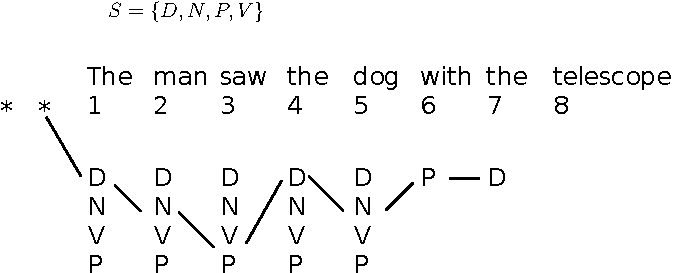
\includegraphics[scale = 0.6]{pics/viterbi1.pdf}
        \end{figure}

\begin{itemize}
 \item There are many possible sequences of tags.
 \item Each of them has a probability calculated from the parameters $q$ and $e$.
 \item $\pi(7, P, D)$ is the maximum probability that one of these tag sequences ends in $P$ $D$ at position $7$.
 \item The path represents the sequence with the maximum probability.
\end{itemize}

\subsection{A Recursive Definition}
  \textbf{Base case:}
  \[
    \pi(0, *, *) = 1
  \]

  \textbf{Recursive definition:}
  For any $k \in \{1 \ldots n\}$, for any $u \in S_{k-1}$ and $v \in S_k$:
  \[
    \pi(k, u, v) = \max_{w \in S_{k-2}} (\pi(k - 1, w, u) \times q(v|w, u) \times e(x_k|v))
  \]


\paragraph{Justification for the Recursive Definition}
  For any $k \in \{1 \ldots n\}$, for any $u \in S_{k-1}$ and $v \in S_k$:
  \[
    \pi(k, u, v) = \max_{w \in S_{k-2}} (\pi(k - 1, w, u) \times q(v|w, u) \times e(x_k|v))
  \]

  
  \begin{figure}[h]
        	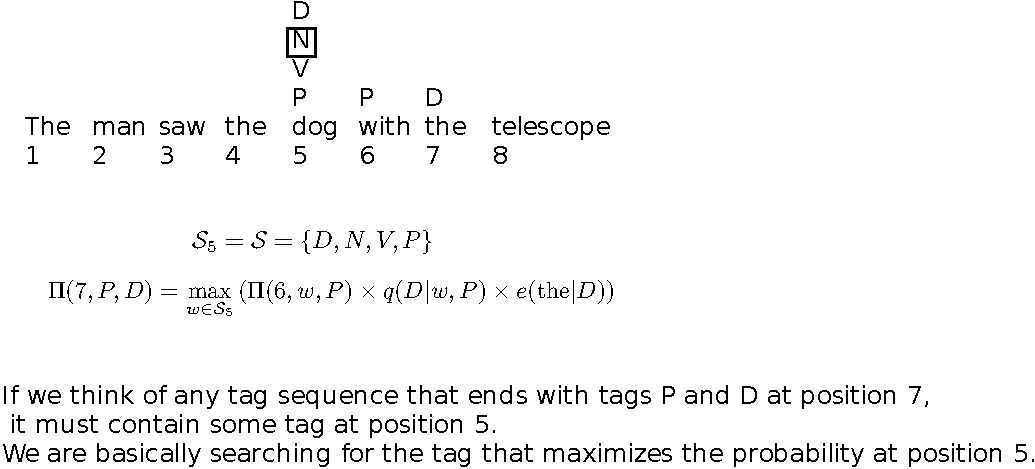
\includegraphics[scale = 0.6]{pics/viterbi2.pdf}
        \end{figure}
        
  \begin{itemize}
   \item Let's consider an arbitrary tag sequence that ends with tags $P$ and $D$ at position $7$.
   \item It must contain some tag at position $5$.
\item We are basically searching for the tag that maximizes the probability at position $5$.
  \end{itemize}
      

\subsection{The Viterbi Algorithm}
\begin{algorithm}[H]
\SetKwInput{Input}{Input}
\SetKwInput{Initialization}{Initialization}
\SetKwFunction{Max}{max}
\SetKwFunction{Return}{return}

\Input{a sentence $x_1 \ldots x_n$, parameters $q(s|u, v)$ and $e(x|s)$}

\Initialization{ Set $\pi(0, *, *) = 1$;  $S_{-1} = S_0 = \{*\}$, $S_k = S$ for $k \in \{1 \ldots n\}$.
}

\BlankLine
\SetAlgoLined
\caption{Viterbi Algorithm}
\label{algo:prob_inference}
\BlankLine

\For{$k = 1$ \KwTo $n$}{
\For{$u \in S_{k-1}, v \in S_k$}{\[\pi(k, u, v) = \max_{w \in S_{k-2}} (\pi(k - 1, w, u) \times q(v|w, u) \times e(x_k|v))\]} 
}



\BlankLine
\Return{$\max_{u \in S_{n-1}, v \in S_n} (\pi(n, u, v) \times q(\text{STOP}|u, v))$} 
\end{algorithm}



\subsection{The Viterbi Algorithm with Backpointers}
\begin{algorithm}[H]
\SetKwInput{Input}{Input}
\SetKwInput{Initialization}{Initialization}
\SetKwFunction{Max}{max}
\SetKwFunction{ArgMax}{argmax}
\SetKwFunction{Return}{return}

\Input{a sentence $x_1 \ldots x_n$, parameters $q(s|u, v)$ and $e(x|s)$}

\Initialization{Set $\pi(0, *, *) = 1$;  $S_{-1} = S_0 = \{*\}$, $S_k = S$ for $k \in \{1 \ldots n\}$.
}

\BlankLine
\SetAlgoLined
\caption{Viterbi Algorithm with Backpointers}
\label{algo:viterbi}
\BlankLine

\For{$k = 1$ \KwTo $n$}{
\For{$u \in S_{k-1}, v \in S_k$}{
\[
\pi(k, u, v) = \max_{w \in S_{k-2}} (\pi(k - 1, w, u) \times q(v|w, u) \times e(x_k|v))
\]    
\[
\text{bp}(k, u, v) = \arg \max_{w \in S_{k-2}} (\pi(k - 1, w, u) \times q(v|w, u) \times e(x_k|v))
    \]} 
}



\BlankLine
$(y_{n-1}, y_n) = \arg \max_{(u,v)} (\pi(n, u, v) \times q(\text{STOP}|u, v))$ \tcp*[r]{Find maximum probability and corresponding tags}
\For{$k = (n - 2)$ \KwTo $1$}{
$y_k = \text{bp}(k + 2, y_{k+1}, y_{k+2})$ \tcp*[r]{Retrieve tag sequence using backpointers}
}

\BlankLine
\Return{the tag sequence $y_1 \ldots y_n$} \tcp*[r]{Return the final tag sequence}
\end{algorithm}



\subsection{The Viterbi Algorithm: Running Time}
  \begin{itemize}
    \item $O(n|S|^3)$ time to calculate $q(s|u, v) \times e(x_k|s)$ for all $k, s, u, v$.
    \item $n|S|^2$ entries in $\pi$ to be filled in.
    \item $O(|S|)$ time to fill in one entry.
  \end{itemize}
  $\Rightarrow$ $O(n|S|^3)$ time in total.

\paragraph{Pros and Cons}
  \begin{itemize}
    \item Hidden Markov Model (HMM) taggers are simple to train (compile counts from training corpus).
    \item They perform relatively well (over 90\% performance on named entity recognition).
    \item Main difficulty is modeling $e(\text{word} | \text{tag})$, which can be very complex if "words" are complex.
  \end{itemize}
